\chapter{Developing the Machine Learning Model}
\label{sec:bearings-model}

\section{Introduction}

In engineering applications, understanding the lifetime of ball bearings is crucial for reliable and efficient operation of machinery. Traditionally, this has been approached through physical models and empirical formulas. However, due to the complexity and numerous factors involved, precise estimation is challenging. Consequently, machine learning offers an alternative approach to address this problem. In this chapter, we will explore the development of a machine learning model to categorize the lifetime of ball bearings based on force (\(F_r\)) and rotational speed (\(n\)). The model will aim to provide a rough estimate of the lifetime, acknowledging that precise prediction is inherently unattainable.

The outline of this chapter is structured to guide through the entire process of model development. Initially, the process of data augmentation through synthetic dataset generation will be discussed, followed by data preprocessing which involves splitting the dataset into training, validation, and test sets. Subsequently, the architecture of the neural network model will be elaborated upon, along with its implementation in PyTorch. The chapter will also delve into the training process, including the configuration of hyperparameters, optimization techniques, and monitoring of the training process. Testing the model's performance and using the model for practical lifetime estimation are also encompassed.

\subsection*{Background on Machine Learning for Categorization}
Machine Learning involves the use of algorithms that can learn from data and make predictions or decisions. In the context of ball bearing lifetime estimation, \ac{ml} can be used to identify patterns in the relationship between variables such as force and rotational speed, and the resulting lifetime. Specifically, categorization or classification can be used to sort lifetime into predefined categories or bins, which is useful in cases where exact predictions are not viable.

\subsection*{Objectives and Requirements of the Machine Learning Model}
The primary objective of the machine learning model developed in this chapter is to categorize the lifetime of ball bearings into bins based on force (\(F_r\)) and rotational speed (\(n\)). The requirements for this model include robustness, generalization to unseen data, and computational efficiency. The model should be able to make reasonably accurate estimations in different scenarios and under various conditions.

In the following sections, the steps and considerations taken to develop a machine learning model to achieve this objective will be discussed in detail.

\section{Generating Datasets}

The success of a machine learning model in making accurate predictions or classifications is heavily influenced by the quality and quantity of the dataset it is trained on. A larger and more diverse dataset is generally more effective in capturing the underlying patterns within the data. This section outlines the procedure and methodology for generating synthetic datasets that replicate the parameters and trends observed in the original dataset, but with an expanded range of values.

\subsection*{Setting Parameters for the Synthetic Dataset}

The first step in generating a synthetic dataset is to set the ranges and intervals for the force (\(F_r\)) and rotational speed (\(n\)) parameters. These parameters can be adjusted to achieve the desired diversity in the dataset. For instance, in the Python script, the ranges for \(F_r\) and \(n\) are defined by the variables \texttt{fr\_range} and \texttt{n\_range} respectively, and the intervals are set through the variables \texttt{fr\_interval} and \texttt{n\_interval}. 

\begin{verbatim}
fr_range = (200, 4000)
n_range = (100, 3500)
fr_interval = 100
n_interval = 100
\end{verbatim}

This configuration generates values for \(F_r\) ranging from 200 to 4000 and values for \(n\) ranging from 100 to 3500, both in increments of 100.

\subsection*{Calculating Lifetime Values}

The synthetic dataset is generated by calculating the lifetime of ball bearings for different combinations of \(F_r\) and \(n\) values. The calculation is based on the refined empirical hypothesis discussed in Chapter 3. The \texttt{generate\_lifetime} function computes the lifetime using the formula:

\begin{verbatim}
def generate_lifetime(fr, n):
    return 4.1378625767 * 10**17 * fr ** (-10/3) * n ** (-1.0)
\end{verbatim}

\subsection*{Clamping the Number of Digits}

In order to keep the dataset consistent with the original, the number of digits in the calculated lifetime values can be limited to 10. This is achieved by the \texttt{clamp\_number} function which takes a number and the total number of digits as input and returns the number rounded to the desired number of digits.

\subsection*{Creating and Saving the Dataset}

Finally, the \texttt{generate\_dataset} function iterates through all combinations of \(F_r\) and \(n\) values within the specified ranges and intervals, calculates the corresponding lifetime using the \texttt{generate\_lifetime} function, and clamps the number of digits. The generated data is then saved in a structured format, usually a CSV file, for later use in training the machine learning model.

This procedure ensures that the synthetic dataset is diverse and covers a broader range of values compared to the original dataset, which is beneficial in training a more robust machine learning model.


\section{Splitting Data into Training, Validation, and Test Sets}

After generating the synthetic dataset, the next critical step in building a machine learning model is to divide the dataset into training, validation, and test sets. This section elaborates on the process and the transformations applied to the data before splitting.

\subsection*{Applying Box-Cox Transformation to Target Variable}

The Box-Cox transformation is a family of power transformations that stabilize variance and make the data more closely follow a normal distribution. The transformation is defined as:

\begin{equation}
y(\lambda) =
\begin{cases}
\dfrac{x^\lambda - 1}{\lambda}, & \text{if }\lambda \neq 0,\\
\log(x), & \text{if }\lambda = 0.
\end{cases}
\end{equation}

where \(y(\lambda)\) is the transformed data, \(x\) is the original data, and \(\lambda\) is the transformation parameter. The optimal value of \(\lambda\) is estimated from the data.

In the Python script, the Box-Cox transformation is applied to the 'Lifetime' column to make the distribution of lifetimes more normal. This can be beneficial for algorithms that make assumptions about the data distribution.

\begin{verbatim}
def apply_boxcox(data, column, save_to_file=False):
    data[column], fitted_lambda = boxcox(data[column])
    ...
\end{verbatim}

\subsection*{Binning the Target Variable}

The target variable \(Lifetime\) is binned into categories using quantiles. This is done to transform the regression problem into a classification problem. Binning based on quantiles ensures that each bin has an approximately equal number of data points. However, it is important to note that if the dataset is not uniformly distributed, this could group values that are far apart.

\begin{verbatim}
def apply_binning(data, column, save_to_file=False):
    data[column], bins = pd.qcut(data[column], q=config["output_size"],
    labels=False, retbins=True, duplicates='drop')
    ...
\end{verbatim}

\subsection*{Normalizing the Features}

Normalizing the features is crucial in ensuring that all features have the same scale. This is important as it can speed up the training process and can also prevent the model from getting stuck in local optima. In this case, the features 'Fr' and 'n' are standardized to have a mean of 0 and a standard deviation of 1 using the StandardScaler of the sklearn library.

\subsection*{Splitting the Dataset}

The dataset is then split into three subsets: training, validation, and test sets. The training set is used for training the model, the validation set is used for tuning hyperparameters and for model selection, and the test set is used to evaluate the performance of the final model.

The \texttt{split\_and\_transform\_dataset} function in the Python script integrates all the above steps. The transformed and split data is saved to CSV files for further processing.

This partitioning is essential to evaluate how well the trained model will generalize to unseen data. Having a separate test set that the model has never seen during training or validation can help to obtain an unbiased estimate of its performance.


\section{Training the Neural Network}

Once the dataset is processed and split into training, validation, and test sets, we proceed to train a neural network. This section discusses the training process, the architecture of the neural network, and the choices made regarding its hyperparameters and functions.

\subsection*{Loading Data}

The training and validation data are loaded from CSV files. These datasets are then split into features (Fr and n) and targets (Lifetime).

\begin{verbatim}
def load_train_data(train_data_path, val_data_path):
  print('Loading data for training and evaluation from csv files...')
  train_data = pd.read_csv(train_data_path)
  val_data = pd.read_csv(val_data_path)
  return train_data, val_data

def split_train_features_targets(train_data, val_data):
  train_features, train_targets = train_data[['Fr', 'n']], train_data['Lifetime']
  val_features, val_targets = val_data[['Fr', 'n']], val_data['Lifetime']
\end{verbatim}

\subsection*{Setting Up the Model}

The neural network is instantiated with an input size of 2 (corresponding to the two features, Fr and n), a hidden layer size of 200, and an output size of 10 (corresponding to the number of bins for the target variable, Lifetime). The activation function used in the hidden layer is \ac{relu}. \ac{relu} is a popular choice for an activation function because it helps in mitigating the vanishing gradient problem and is computationally efficient \cite[p. 111]{ketkar21}.

\begin{verbatim}
class LifetimeModel(nn.Module):
  def __init__(self, input_size, hidden_size, output_size, activation_function):
      super(LifetimeModel, self).__init__()
      self.linear1 = nn.Linear(input_size, hidden_size)
      self.activation_function = activation_function
      self.linear2 = nn.Linear(hidden_size, output_size)

  def forward(self, x):
      output = self.linear1(x)
      output = self.activation_function(output)
      output = self.linear2(output)
      return output

model = LifetimeModel(input_size=2, hidden_size=200, output_size=10, activation=nn.ReLU())
\end{verbatim}

\subsection*{DataLoaders}

DataLoaders are used to efficiently load and process the training and validation datasets. The batch size is set to 64, which means that the model is updated after processing 64 samples. This is a trade-off between computational efficiency and the granularity of updates. Shuffling is enabled for the training set to ensure that the model does not learn any order dependencies from the dataset. Pin memory is enabled for faster data transfer from CPU to GPU.

\begin{verbatim}
class BearingDataset(Dataset):
  def __init__(self, features, targets):
      self.data = torch.tensor(features, dtype=torch.float32)
      self.target = torch.tensor(targets, dtype=torch.long)

  def __len__(self):
      return len(self.data)

  def __getitem__(self, idx):
      return self.data[idx], self.target[idx]

train_dataloader = DataLoader(train_dataset, batch_size=config["batch_size"],
shuffle=True, pin_memory=True)
val_dataloader = DataLoader(val_dataset, batch_size=config["batch_size"],
shuffle=True, pin_memory=True)
\end{verbatim}

\subsection*{Optimizer and Loss Function}

The Adam optimizer is used with a learning rate of 0.001. Adam is an adaptive learning rate optimization algorithm that has been shown to work well in practice. The learning rate determines how large the updates to the model parameters are during training.

The loss function used is Cross-Entropy Loss, which is suitable for classification problems. This loss function measures the dissimilarity between the predicted probability distribution and the actual distribution.

\begin{verbatim}
optimizer = torch.optim.Adam(model.parameters(), lr=0.001)
loss_fn = nn.CrossEntropyLoss()
\end{verbatim}

\subsection*{Training Process}

The model is trained for 1000 epochs. An epoch is one complete pass through the entire training dataset. During each epoch, the model's parameters are updated to minimize the loss function. The forward pass involves passing the input through the network and computing the output. The backward pass involves computing the gradient of the loss with respect to the model parameters and updating the parameters.

Validation is performed every 10 epochs to check the model's performance on unseen data. This helps in monitoring for overfitting and can be used for hyperparameter tuning.

\begin{verbatim}
def train_model(train_dataloader, val_dataloader, model, loss_fn,
optimizer, epochs, device):
  for epoch in range(1, epochs + 1):
      for inputs, targets in train_dataloader:
          inputs, targets = inputs.to(device), targets.to(device)
          # Forward pass
          outputs = model(inputs)
          loss = loss_fn(outputs, targets)

          # Backward pass and optimization
          optimizer.zero_grad()
          loss.backward()
          optimizer.step()

      # Validate the model
      if epoch % 10 == 0:
          val_loss = 0
          val_acc = 0
          with torch.no_grad():
              for inputs, targets in val_dataloader:
                  inputs, targets = inputs.to(device), targets.to(device)
                  outputs = model(inputs)
                  _, predicted = torch.max(outputs, 1)
                  val_loss += loss_fn(outputs, targets)
                  val_acc += (predicted == targets).sum().item()
\end{verbatim}

After training, the model's parameters are saved to a file for future use.

\subsection*{Device Choice}

Usually, for training neural networks, CUDA-enabled GPUs are preferred due to their significantly higher computational capabilities compared to CPUs, especially for large models and datasets. CUDA is a parallel computing platform and API model created by NVIDIA, and it allows for leveraging the computing power of NVIDIA GPUs.

However, in this particular instance, the dataset is relatively small. Upon measuring the time taken for training on both CPU and CUDA-enabled GPU, it was observed that the CPU was faster. This can be attributed to the overhead involved in transferring data to the GPU memory and the relatively small size of the model, which does not fully utilize the parallel processing capabilities of the GPU.

Moreover, utilizing CUDA requires a GPU from NVIDIA that supports this technology. On the other hand, there is an alternative for AMD GPUs called ROCm, but as of the writing of this document, it is not yet properly supported on Windows operating systems.

In the script, the device choice can be configured using the \verb|prefer_cuda| option in the config dictionary.

\begin{verbatim}
device = torch.device("cuda" if torch.cuda.is_available()
and prefer_cuda else "cpu")
\end{verbatim}

The flexibility in device choice allows for optimizing the training process depending on the hardware and dataset characteristics.

\subsection{Testing the Model}

After training the model, it is essential to evaluate its performance on unseen data to assess its generalization capability. For this, we employ two metrics: overall accuracy and a confusion matrix. The code provided tests the model on a separate test dataset and produces a confusion matrix as output.

\subsubsection{Overall Accuracy}

The overall accuracy provides a rough estimate of the model's performance by calculating the percentage of correct predictions. In this particular case, the model achieved an accuracy of 96.7\%, with 264 out of 273 predictions being correct on the test dataset. However, overall accuracy doesn't provide detailed information about the nature of the mistakes made by the model \cite[p. 148 ff.]{ketkar21}.

\subsubsection{Confusion Matrix}

While overall accuracy is informative, it is often more useful to analyze the confusion matrix for a more detailed understanding of the model's performance. The confusion matrix reveals not only the number of correct and incorrect predictions but also how these predictions are distributed across the different classes. In the confusion matrix, the rows represent the actual classes, and the columns represent the predicted classes. The diagonal elements of the matrix represent the number of points for which the predicted label is equal to the true label, while the off-diagonal elements are those that are mislabeled by the classifier.

\begin{figure}[h]
    \centering
    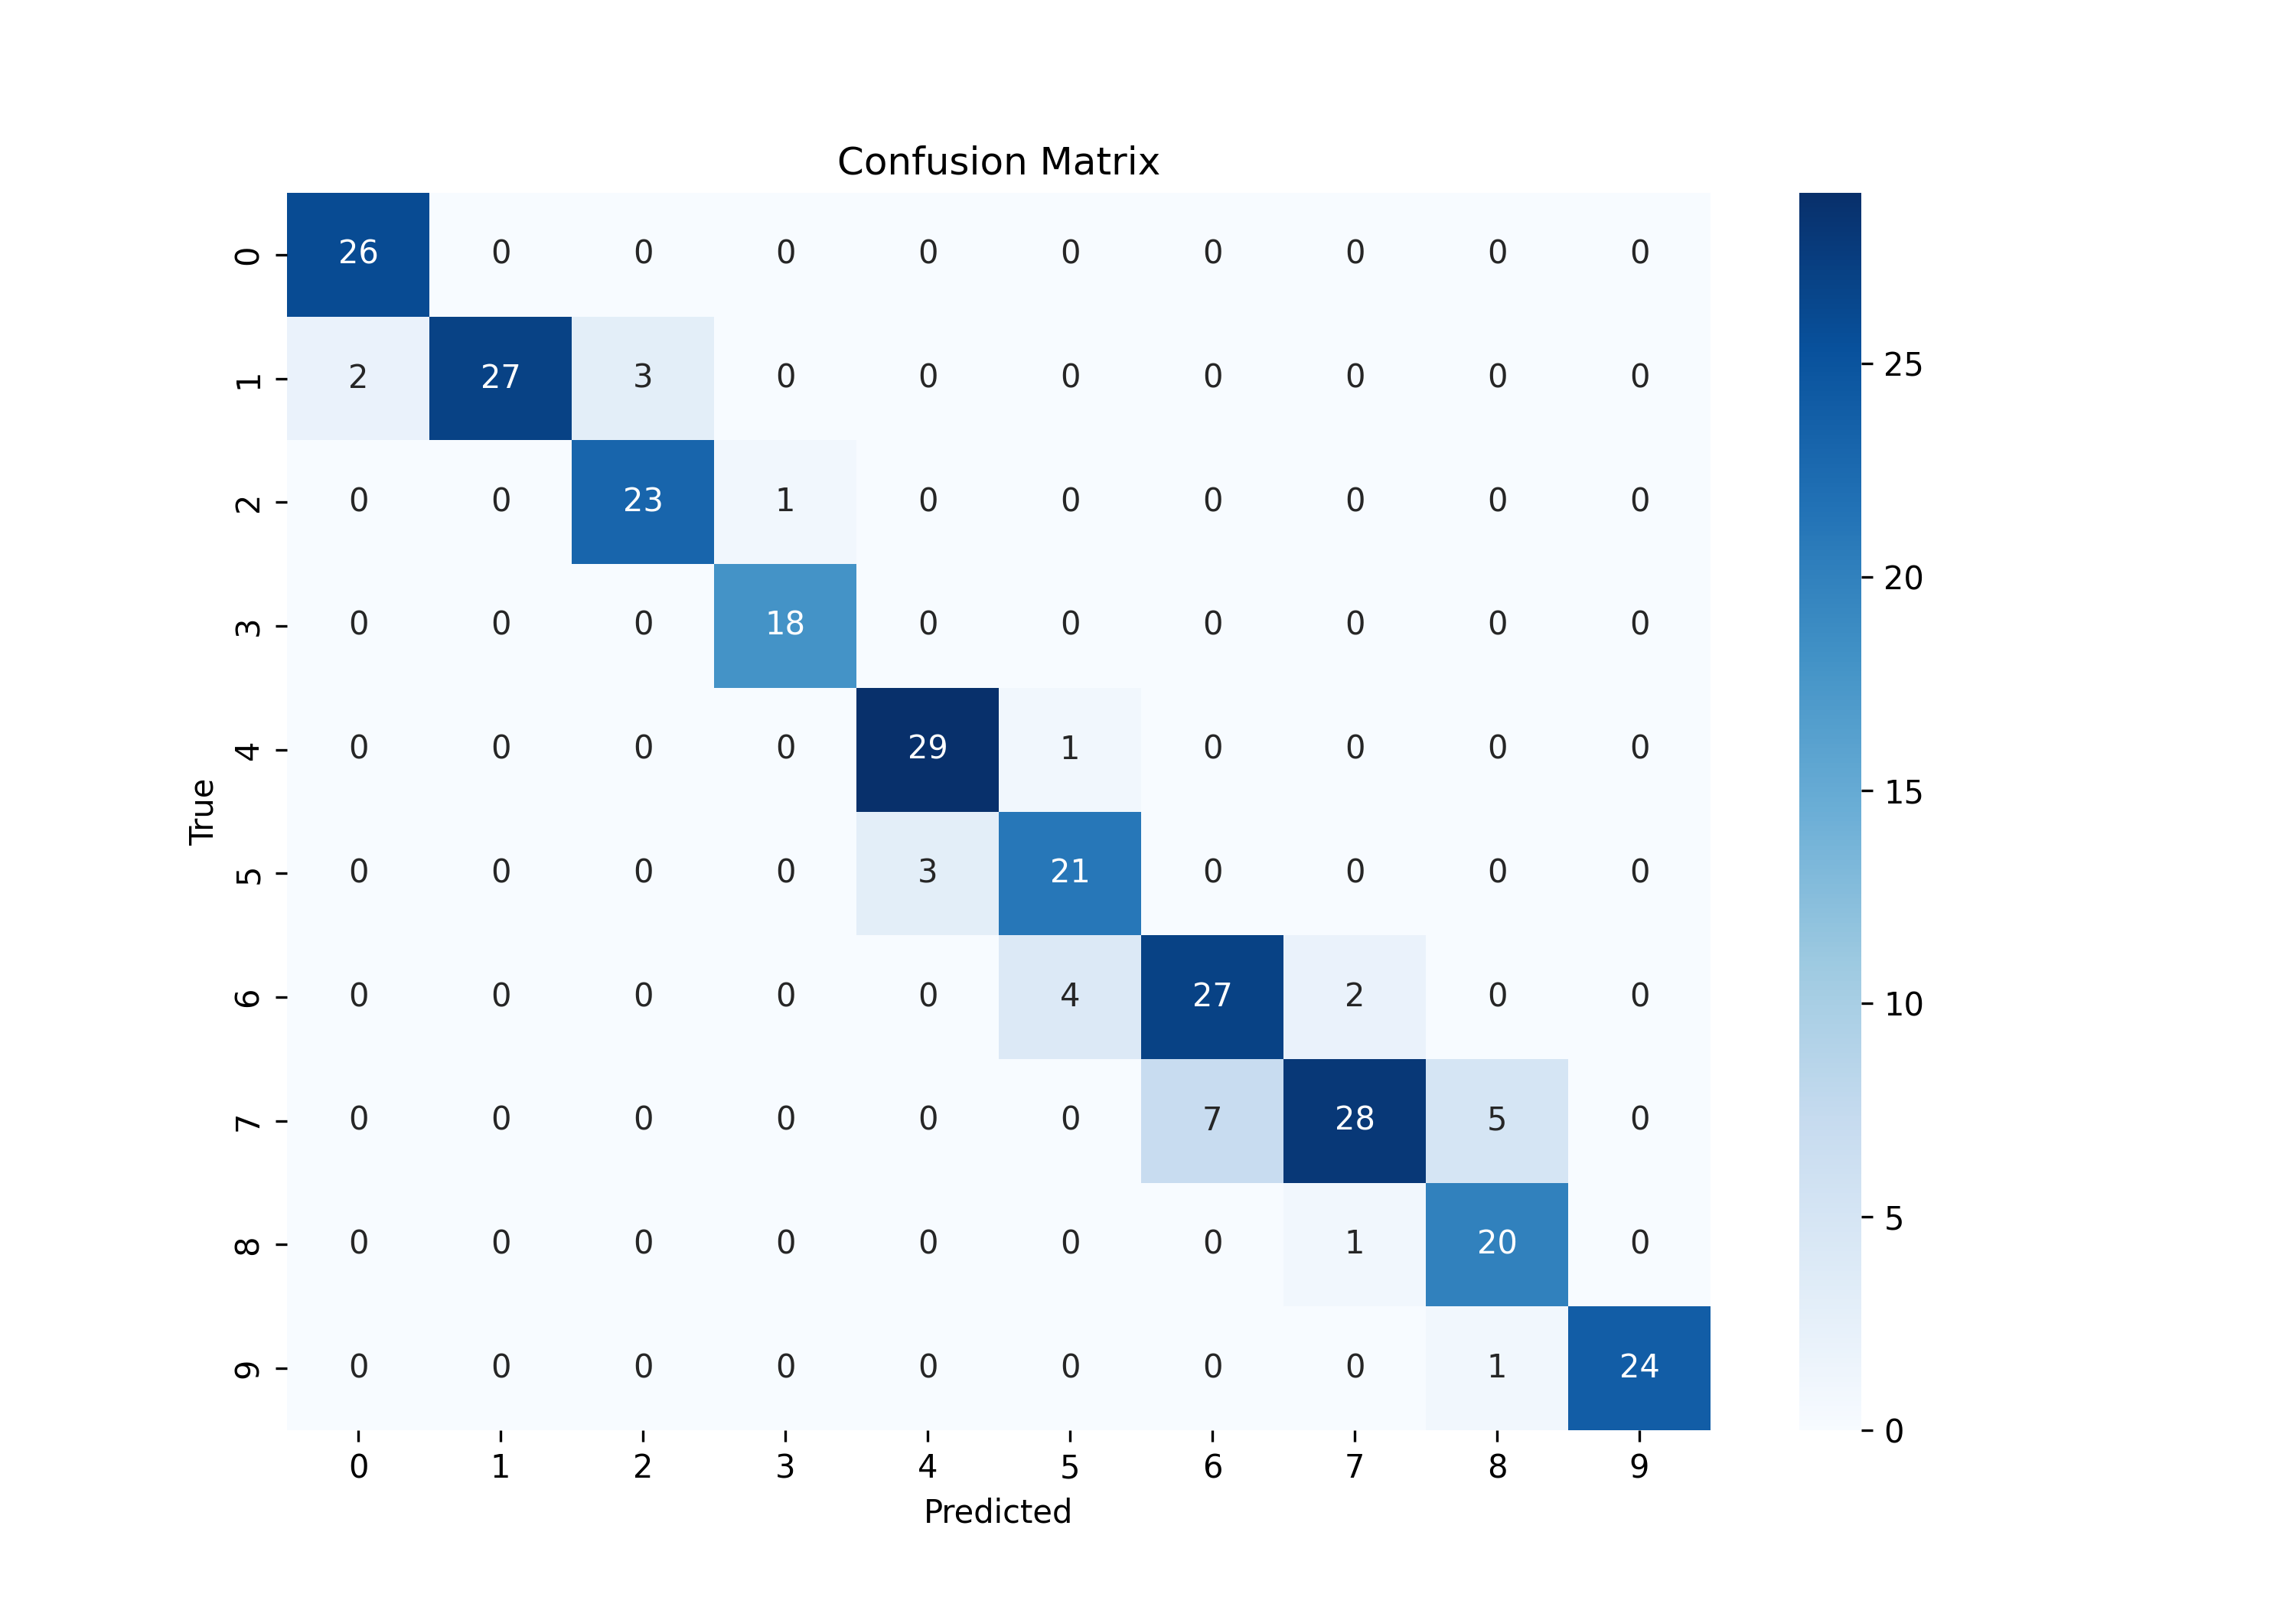
\includegraphics[width=0.8\linewidth]{assets/bearings-model/confusion-matrix.png}
    \caption{Confusion Matrix illustrating the performance of the model.}
    \label{fig:confusion_matrix}
\end{figure}

From the confusion matrix, it is evident that most of the predictions are on the diagonal, indicating that they are correct. Importantly, the incorrect predictions are located within one bin of the correct answers. This means that, even when the model is incorrect, it is not far off from the true value, which is a very positive sign. 

\subsubsection{Implications and Interpretation of the Confusion Matrix}

The confusion matrix reveals that the model has a high predictive accuracy and that the mistakes it makes are minor. One factor contributing to this high accuracy is that the test data is in the same distribution as the training data. In the real world, this is not considered to be a significant issue for this application, as the values for frequency and RPM usually fall within this range.

This is particularly encouraging for the application in predicting the lifetime of bearings based on frequency and \ac{rpm}, as even a slight misprediction doesn't drastically affect the interpretability or usability of the model's output. 

Knowing that errors are close to the true values allows for some flexibility in using this model in practical applications. It might be reasonable to make decisions based on a range of values rather than a specific point estimate. 

The model's high accuracy, coupled with the minor nature of its errors, indicates that it is well-suited for practical applications. However, it is important to keep in mind that the model's performance is partly due to the similarity in the distribution between the training and test datasets. Real-world data may still vary, so it's important to continually monitor the model's performance and make necessary adjustments as required.


\subsection{Estimating Lifetime Using the Model}
In practical applications, the typical use case of the model is to estimate the Lifetime of a bearing given its frequency and rotational speed. To facilitate this, a script has been developed that takes these two features as input and outputs the estimated Lifetime.

\subsubsection{Data Transformation and Prediction}
The script starts by loading the model, the scaler, and the parameters for the Box-Cox transformation that were saved during the training phase. The user is then prompted to input the values for \(Fr\) and \(n\). The input features are normalized using the scaler, which is crucial since the model was trained on normalized data.

The model estimates the Lifetime category (bin) corresponding to the input features. Additionally, the script calculates the Lifetime using the formula derived in Chapter \ref{sec:bearings-hypothesis} as a benchmark. The calculated Lifetime is then transformed into a bin after applying the Box-Cox transformation with the same lambda parameter that was fitted on the training data. This ensures consistency between the transformations applied to the dataset and the input values.

\subsubsection{Preliminary Results}
Preliminary tests with sample data have shown promising results. The model's estimates are reasonable, and the predicted Lifetime categories are consistent with the actual Lifetime calculated using the formula.

However, it's essential to understand that these tests are preliminary and not exhaustive. Further testing with a wider range of data is necessary to ascertain the model's reliability and accuracy in real-world applications.

\subsubsection{Future Testing}
As the model begins to be employed in real-world scenarios, it will be imperative to continuously monitor its predictions and evaluate its performance. There might be a need for further tuning or even retraining the model with additional data as more information becomes available.

Additionally, practical applications may involve more complex conditions than those in the training data, and the model should be robust enough to handle such variations. Ongoing validation and updates are key to ensuring the model remains effective and valuable in its intended applications.
